\documentclass[a4paper, 10pt, english, oneside]{extarticle}
../mwe/preamble.tex

\author{Roxana Pamfil} 
\title{Community Structure In Product-Purchase Networks} 
\myface{roxana_face} 

\begin{document}
\maketitle % Make the title. 

I am Roxana Pamfil, a former InFoMM student from Cohort 1. My
DPhil was in the area of network science and was in collaboration
with dunnhumby, a customer data science company headquartered
in London. After my DPhil, I received 6 months of funding from both
dunnhumby and Oxford to work as ``Knowledge Transfer Ambassador''
and help dunnhumby apply my research to their business
problems. This was a unique opportunity to see an immediate impact
of my DPhil work outside of academia and to bring new expertise
to the company’s data scientists.

My DPhil research was about community detection, a form of clustering
in networks. A network is an abstract representation of a system
in which objects called nodes interact with each other pairwise
via edges. For my collaboration with dunnhumby, I have studied networks of customers connected
to previously-purchased grocery products (see \Cref{network}). This is an example of a bipartite network,
in which edges connect nodes of different types. By predicting edges in such a network, we can
address two important business problems:
\begin{enumerate}
\item {} [Recommendations] What new items should we recommend to a given customer?
\item {} [Targeting] Which users should we contact in a promotional campaign for a specific product?
\end{enumerate}


\begin{SCfigure}[][htb]
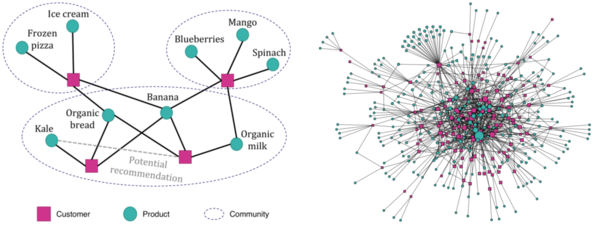
\includegraphics[width=0.7\linewidth]{network}
\caption{\textbf{(Left)} Diagram of a
customer–product
network.
\textbf{(Right)} A larger bipartite
network.}
\label{network}
\end{SCfigure}

\section*{Promotional targeting}

My proposed targeting solution consists of 5 steps (see \Cref{flow_chart}). After
constructing a network from the raw data, detecting communities, and fitting a statistical model,
we can calculate the probability of an edge existing between any customer and product. The top
customers according to these probabilities can then be sent coupons to elicit an initial purchase
of the product on promotion.

\begin{figure}[h!tb]
\centering
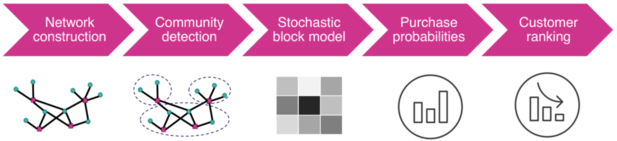
\includegraphics[width=0.7\linewidth]{flow_chart}
\caption{Key steps in a network-science approach to targeting.}
\label{flow_chart}
\end{figure}

For this approach to be of practical use to dunnhumby, it needs to scale to data sets of millions of customers and tens of thousands of products. Community detection is the most computationally-intensive step in the process, so a key task for me was to compare different algorithms. I found that a Python package called leidenalg provides a good balance between accuracy and speed; it runs in a few hours on a customer-product network with half a billion edges.

I validated this targeting approach using historical transactions and promotional campaigns that were previously run by dunnhumby. These results suggest that we can capture a customer's affinity for a product based on their similarity to other customers within their community. This is especially useful for acquisition customers, who are new or infrequent buyers of the product on offer. Based on these initial results, there is interest within dunnhumby to test the approach in a live campaign. To facilitate this process, I made my code available through a Python package for bipartite network analysis.

\begin{figure}[htb]
\centering
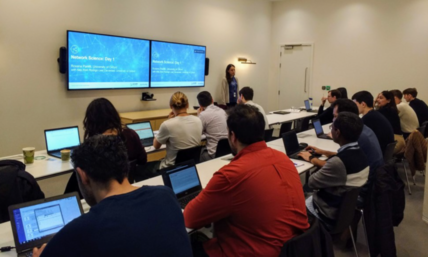
\includegraphics[height=0.17\paperheight]{classroom}
\hfill 
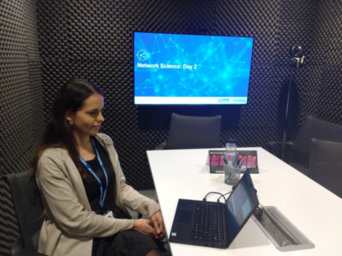
\includegraphics[height=0.17\paperheight]{roxana_laptop}
\caption*{Roxana teaching network science to dunnhumby’s data scientists.}
\end{figure}

\section*{Network science course}

The intention with this course was to expand the toolkit of dunnhumby's data scientists to include common tools for network analysis. The course was a combination of lectures and hands-on Python exercises delivered over 1.5 days. To ensure an emphasis on topics relevant to dunnhumby, I suggested possible use cases within the business of the methods that I presented, and I created several exercises which involved the analysis of networks constructed from transaction data.

The initial plan was to run this course once, in dunnhumby's London office. Due to considerable interest in the topic, I ended up delivering the course 5 times, to around 80 participants working in London, Manchester, India, and the US. The course was well-received, with an overall rating of 4.4 out of 5. Attendees appreciated the breadth of topics covered and the availability of Python code that they could reuse later. A few participants were keen to use what they had learned right away and reached out to me after the course with further questions.


On a personal level, working on this project taught me a few things that will serve me well in the future. I was never told what to do. Instead, I had to manage my own work (with some input from supervisors), set my own deadlines, and solve any issues that came up. In many ways, I had a level of responsibility in this project that is more common at later stages in one's career. While my collaboration with dunnhumby ends here, I hope that they will be able to use my work for many years to come.

\end{document}